\subsection{Grandes oscilações: abertura dinâmica}\label{sec:3.6}
O campo guia de um anel de armazenamento normalmente aceita apenas uma pequena faixa de energias -- tipicamente só uma pequena porcentagem da energia nominal -- e as forças magnéticas focalizadoras são razoavelmente lineares em toda esta faixa de energia. No entanto, pequenos desvios de energia podem corresponder a grandes oscilações do deslocamento temporal $\tau$. Neste caso, grandes oscilações significam valores de $\tau$ onde $V(\tau)$ deixa de ter uma dependência linear com $\tau$. Estas grandes amplitudes ocorrem geralmente quando a tensão de pico de RF não é muito maior que a perda por radiação (que é o caso em altas energias) ou quando o número harmônico de RF $k$ é muito grande. Estas oscilações devem ser analisadas pois são elas as responsáveis por determinar a abertura dinâmica do anel. Mantenha em mente que, apesar de grandes oscilações temporais estarem sob análise, as oscilações de energia continuam pequenas.

Pois bem, da \autoref{sec:3.4} foram obtidas as equações \eqref{eq:3.32} e \eqref{eq:3.34}. Como foi feito antes, substitui-se $U_{rad}$ por $U_0 +D\epsilon$, já que as oscilações de energia são pequenas. Mas agora $V(\tau)$ não pode mais ser substituída por sua aproximação linear, então a equação \eqref{eq:3.34} fica
\begin{align}
	\frac{d\epsilon}{dt} = \frac{eV(\tau) - U_0}{T_0} - \frac{D\epsilon}{T_0}
\end{align}
Expressando $\epsilon$ e sua derivada com relação ao tempo em termos de $\tau$ pela equação \eqref{eq:3.32}, tem-se
\begin{align}
	\frac{d^2 \tau}{dt^2} = -\frac{\alpha}{E_0 T_0}[eV(\tau)-U_0] - \frac{D}{T_0}\frac{d\tau}{dt}\label{eq:3.49}
\end{align}
Esta equação descreve a variação de $\tau$ para qualquer amplitude.

É possível comparar a equação \eqref{eq:3.49} com uma equação bem conhecida:
\begin{align}
	m\frac{d^2x}{dt^2} = F(x) - \mu\frac{dx}{dt}\label{eq:3.50}
\end{align}
Esta equação representa o movimento unidimensional em $x$ de uma partícula com massa $m$, a qual se move em um campo de força conservativo $F(x)$ e sofre uma força de fricção proporcional à sua velocidade. Sendo assim, pode-se entender a equação \eqref{eq:3.49} por meio de uma comparação direta com a equação \eqref{eq:3.50}. O movimento em $\tau$ é exatamente igual ao movimento de uma partícula com massa unitária em um campo de força conservativo
\begin{align}
	F(\tau) = -\frac{\alpha}{E_0 T_0}[eV(\tau) - U_0]\label{eq:3.51}
\end{align}
sofrendo uma força de fricção proporcional à sua velocidade com um coeficiente $D/T_0$.

Geralmente, o movimento em $\tau$ pode ser avaliado apenas por computação numérica. No entanto, pode-se obter uma boa ideia heurística considerando o que acontece se o termo friccional é zero. Ele é mesmo pequeno e pode ser considerado como uma perturbação depois. Pois bem, deseja-se estudar o movimento
\begin{align}
	\frac{d^2\tau}{dt^2} = F(\tau)
\end{align}
onde $F(\tau)$ é dada pela equação \eqref{eq:3.51}. Este tipo de equação é geralmente resolvido definindo uma função de "energia potencial", a qual é o negativo da integral da força. Assim, define-se
\begin{align}
	\Phi(\tau) = \frac{\alpha}{E_0 T_0} \int\limits_{\tau}^{0}[eV(\bar{\tau}) - U_0]d\bar{\tau}
\end{align}
Agora o movimento pode ser analisado utilizando o princípio de conservação de energia. Em cada instante, a soma da "energia potencial" $\Phi(\tau)$ e da "energia cinética" -- dada por $\frac{1}{2}(d\tau/dt)^2$ -- deve ser constante, dada pela "energia total". A energia total também é o máximo $\Phi_0$ que pode ser alcançado por $\Phi(\tau)$ -- o qual irá ocorrer quando $d\tau/dt$ for zero. Logo, pode-se escrever que
\begin{align}
	\frac{1}{2}\left(\frac{d\tau}{dt}\right)^2 = \Phi_0 - \Phi(\tau)\label{eq:3.54}
\end{align}

Suponha que a função do ganho de energia $eV(\tau)$ tenha a forma representada na \autoref{fig:fig36}(a) e o ganho de energia síncrono $U_0$ também representado nesta figura. Então $\Phi(\tau)$ será como a curva representada na parte (b) da \autoref{fig:fig36}. A forma mostrada é razoavelmente típica. Note que $\Phi(\tau)$ tende a decrescer com uma inclinação média de $-U_0$. Isto precisa ocorrer pois a integral dos campos de aceleração de RF deve ser zero em um ciclo completo (pelo menos em um ciclo completo da menor frequência presente).

\begin{figure}[!htb]
	\centering
	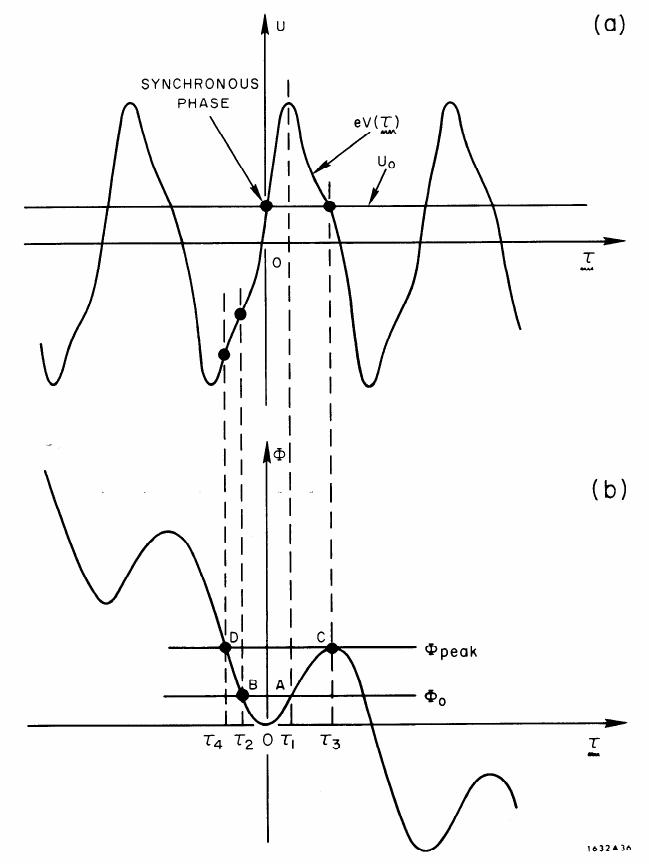
\includegraphics[width=0.9\linewidth]{./Figuras/fig36.jpeg}
	\caption{(a) Função de aceleração de RF $eV(\tau)$, e (b) a função da energia potencial efetiva $\Phi(\tau)$.}
	\label{fig:fig36}
\end{figure}

Agora a natureza das oscilações do deslocamento temporal pode ser visualizada. O movimento é parecido com o de uma partícula pontual (um "elétron") que se move "pela" superfície montanhosa representada por $\Phi(\tau)$ -- onde, é claro, você deve pensar em $\tau$ como sendo uma coordenada espacial horizontal. Primeiramente, existe um potencial mínimo em $\tau=0$. Se o elétron é posicionado neste ponto, ele permanece estacionário; este é o "elétron síncrono" \footnote{Existem, é claro, pontos estacionários em cada mínimo do potencial, e estes correspondem aos elétrons síncronos nos centros de outros \textit{bunches} (enquanto $\tau<T_0$).}. No entanto, se o elétron for posicionado em $\tau_1$ -- o ponto correspondente ao ponto $A$ na montanha -- ele irá descer pela montanha e para no ponto oposto B. A e B estão na mesma altura $\Phi_0 = \Phi(\tau_A)$. Em $\tau_A$ e $\tau_B$ a energia cinética é zero. A energia cinética irá atingir seu valor máximo quando o elétron passar $\tau=0$. Em cada $\tau$ a energia cinética é dada pela equação \eqref{eq:3.54} e a partir desta pode-se obter a "velocidade" em cada $\tau$:
\begin{align}
	\frac{d\tau}{dt} = \pm \sqrt{2}[\Phi_0 - \Phi(\tau)]^{1/2}
\end{align}

Lembre-se, agora, que pela equação \eqref{eq:3.32} a "velocidade" é dada por
\begin{align*}
	\frac{d\tau}{dt} = -\alpha \frac{\epsilon}{E_0}
\end{align*}
então o desvio de energia (de um elétron real) em cada $\tau$ é dado por
\begin{align}
	\frac{\epsilon(\tau)}{E_0} = + \frac{\sqrt{2}}{\alpha}[\Phi_0-\Phi(\tau)]^{1/2}\label{eq:3.56}
\end{align}

Esta relação pode ser facilmente vista em um diagrama de fase -- $\epsilon$ versus $\tau$ -- no qual quase uma elipse é obtida, semelhante à curva representada na \autoref{fig:fig37}. Deve-se apenas utilizar o senso comum para escolher o sinal apropriado da raiz quadrada para cada metade do ciclo.

\begin{figure}[!htb]
	\centering
	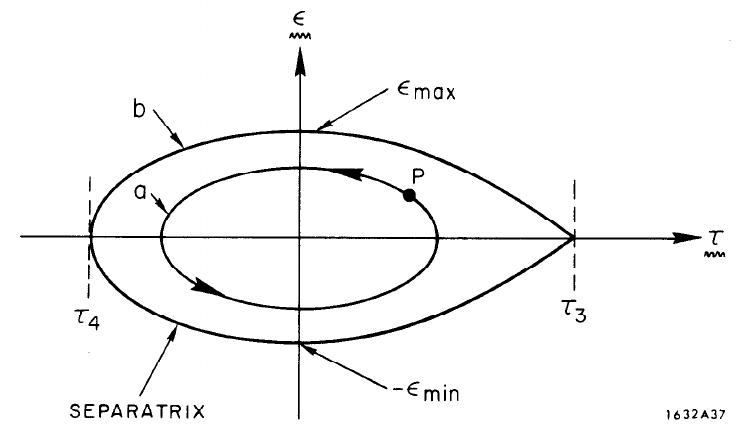
\includegraphics[width=0.7\linewidth]{./Figuras/fig37.jpeg}
	\caption{Diagrama de fase para grandes oscilações. Oscilações de energia limitadas ocorrem apenas dentro da separatriz.}
	\label{fig:fig37}
\end{figure}

Também pode-se ver o que acontece considerando o termo de fricção -- o amortecimento por radiação. Durante cada ciclo de oscilação, uma pequena quantidade de energia será perdida, resultando numa diminuição da "energia" total (pode-se estimar este valor se o movimento for aproximado por uma senoide).

Deve ser aparente que haverá uma amplitude máxima para as oscilações estáveis (periódicas) de $\tau$. Ela ocorre quando o elétron atinge o pico da montanha em $\tau_3$ -- correspondente ao ponto C da \autoref{fig:fig36}(b) -- onde $\Phi(\tau)$ é $\Phi_{max}$. Um elétron com qualquer amplitude maior irá passar o pico da montanha e adentrar o vale seguinte, onde ele terá tanta "energia cinética" que continuará neste movimento para sempre -- até que ele se perca no anel de armazenamento.

As oscilações estáveis máximas variam entre os pontos C e D. Note que o ponto C também é o ponto onde $eV(\tau)$ é igual a $U_0$ novamente (à esquerda de C o elétron real sempre ganha energia e pode ainda ter esperança de retornar ao seu $\tau$ original). O outro extremo da oscilação no ponto D não tem nenhuma característica especial exceto que $\Phi(\tau)$ é igual a $\Phi_{max}$ novamente, o valor em C. O diagrama de fase para grandes oscilações é um pouco peculiar, já que tanto a velocidade quanto a aceleração vão para zero em C mas não em D. O elétron "permanece" em C -- no caso ideal para um tempo infinito! Como resultado, o diagrama de fase tem uma "quina", a qual é mostrada na curva b da \autoref{fig:fig37}. Esta curva especial é chamada de \uline{separatriz} porque ela separa as oscilações estáveis das instáveis. Um elétron injetado num anel de armazenamento com um certo desvio de energia $\epsilon$ e deslocamento no tempo $\tau$ correspondentes ao ponto P na \autoref{fig:fig37} irá circular em uma trajetória fechada mais ou menos elíptica (desconsiderando o amortecimento). Se um elétron é injetado fora da separatriz, ele será "perdido".

Agora, pode-se analisar como o sistema de RF pode determinar a abertura dinâmica do anel de armazenamento. Desvios de energia maiores que $\pm \epsilon_{max}$ -- na \autoref{fig:fig37} -- não podem ser armazenados no anel. Elétrons podem ser perdidos em desvios de energia menores se seus deslocamentos laterais $x_\epsilon$ associados a $\epsilon$ fizerem com que o elétron colida com alguma barreira física que limita a abertura radial. Normalmente, no entanto, a limitação da RF que determina a abertura dinâmica $\pm \epsilon_{pico}$. Da equação \eqref{eq:3.56}
\begin{align}
	\frac{\epsilon_{max}}{E_0} = \frac{1}{\alpha}[2\Phi_{max}]^{1/2}
\end{align}

Se você analisar $\Phi(\tau)$ no caso especial que a tens]ao de RF é senoidal -- ou seja, descrita pela \eqref{eq:3.36} -- obtém-se que
\begin{align}
	\Phi_{max} = \frac{\alpha U_0}{2\pi k E_0} F(q)
\end{align}
onde
\begin{align}
	q = e\widehat{V}/U_0
\end{align}
é a sobretensão -- a taxa da tensão de pico de RF para a tensão mínima necessária para armazenar um elétron síncrono -- e
\begin{align}
	F(q) = 2\left[\sqrt{q^2 - 1} - cos^{-1}(1/q)\right]
\end{align}
A abertura dinâmica $\epsilon_{max}$ para este caso é dada por
\begin{align}
	\left(\frac{\epsilon_{max}}{E_0}\right)^2 = \frac{U_0}{\pi \alpha k E_0} F(q)
\end{align}

A função da abertura dinâmica $F(q)$ é representada na \autoref{fig:fig38}. Note que para $q$ grande
\begin{align}
	F(q) \rightarrow 2q-\pi
\end{align}

\begin{figure}[!htb]
	\centering
	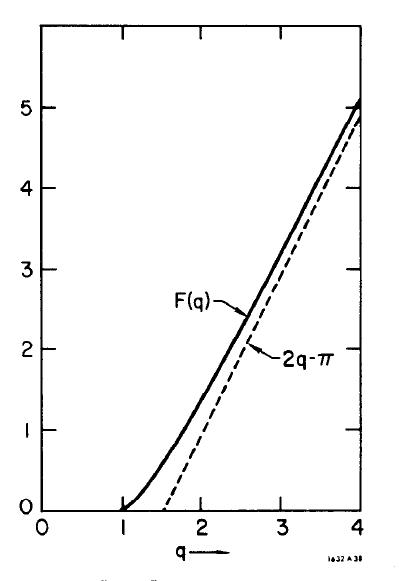
\includegraphics[width=0.5\linewidth]{./Figuras/fig38.jpeg}
	\caption{Função da abertura dinâmica $F(q)$.}
	\label{fig:fig38}
\end{figure}

Finalmente, pensando no que acontece se um elétron inicia fora da abertura dinâmica --  diga-se em pontos acima do ponto D na curva de $\Phi(\tau)$ na \autoref{fig:fig36}(b) -- e descobrindo qual seria sua trajetória de fase, o resultado seriam as curvas da \autoref{fig:fig39}. três separatrizes sucessivas são mostradas e diversos exemplos de trajetórias instáveis. Novamente, observa-se que um elétron que começa sua trajetória fora de uma região estável irá -- exceto por um fortuno acidente -- ficar fora para sempre.

\begin{figure}[!htb]
	\centering
	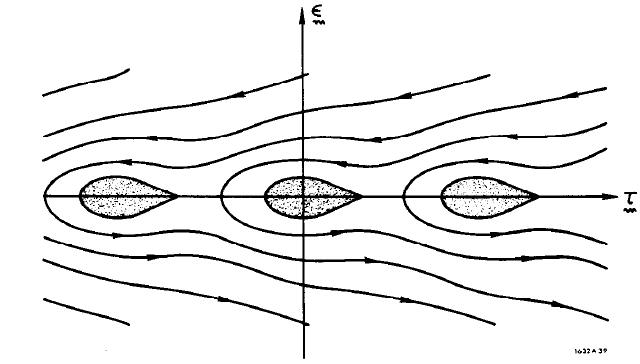
\includegraphics[width=0.7\linewidth]{./Figuras/fig39.jpeg}
	\caption{Trajetórias de fase para elétrons não capturados em um \textit{bunch} (um desenho qualitativo).}
	\label{fig:fig39}
\end{figure}